% This is samplepaper.tex, a sample chapter demonstrating the
% LLNCS macro package for Springer Computer Science proceedings;
% Version 2.20 of 2017/10/04
%




\documentclass[runningheads]{llncs}
%
\usepackage{graphicx}
\usepackage{lipsum}
\usepackage{amsmath}
\usepackage{authblk}
\usepackage{makecell,array}
%\usepackage{natbib}
%\usepackage[square,sort,comma,numbers]{natbib}
%\usepackage[numbers]{natbib}
\usepackage[square,numbers]{natbib}
\usepackage{graphicx}
\usepackage{float}
\usepackage{gensymb}
% Used for displaying a sample figure. If possible, figure files should
% be included in EPS format.
%
% If you use the hyperref package, please uncomment the following line
% to display URLs in blue roman font according to Springer's eBook style:
% \renewcommand\UrlFont{\color{blue}\rmfamily}

\begin{document}
	%
	\title{Coursera - IBM Data Science Specialization Capstone Project}
	% Prediction of Interests of new Rental Listing Inquiries
	%
	%\titlerunning{Abbreviated paper title}
	% If the paper title is too long for the running head, you can set
	% an abbreviated paper title here
	%
	%
    \author{Sebastian Mack}
	% First names are abbreviated in the running head.
	% If there are more than two authors, 'et al.' is used.
	%
	\institute{Sebastian Mack \and
		\email{mack.seb@gmail.com}}
	%
	\maketitle              % typeset the header of the contribution
	
	\begin{abstract}
		
	
		\keywords{Data Science \and Prediction \and GBM \and Tuning.}
	\end{abstract}
	
	\newpage
	%
	%

	\section{Introduction}
	The background for this capstone project is to have the opportunity to be as creative as possible and come up with ideas to leverage the Foursquare location data to come up with a problem that can use the Foursquare location data to solve. 
	
	\subsection{Project Overview}

	As the field of study I selected an interesting topic from the rental industry that caught my attention when I was exploring topics on the data science platform Kaggle. The initiator of this contest is RentHop (a portfolio company of Two Sigma Ventures) which has the objective to make apartment search smarter by using data to sort rental listings by quality (refer to \url{https://www.renthop.com/}).
	
	\begin{figure}[h]
      \centering
      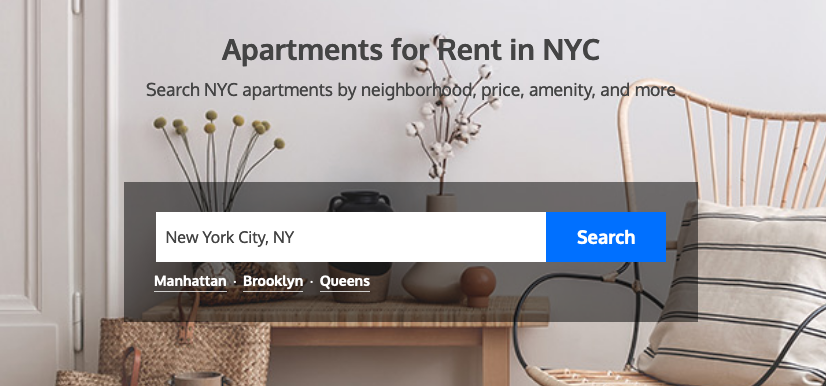
\includegraphics[width=300pt]{rent.png}
      \caption{Renthop Platform}
      \label{fig:rent}
    \end{figure}
    
    \subsection{Problem Statement}
In this project we want to predict how popular an apartment rental listing is based on the listing content like text description, photos, number of bedrooms, price, etc. The data comes from renthop.com, an apartment listing website. These apartments are located in New York City.
The target variable, interest\_level, is defined by the number of inquiries a listing has in the duration that the listing was live on the site. 

For me personally this problem is very interesting because it represents a real life problem that not only Renthop but many other companies are facing right now. In this situation companies are already acquiring and collecting data with their existing services but still struggle to create a business value out of it. In this particular case we can see that by developing a model that can predict how much interest a new rental listing on RentHop will receive, new business values can be proposed. Both the consumer and the merchants could benefit from such a situation. Furthermore the offering company could gain new clients with this value adding service.
\newline

\subsection{Approach}
The problem that is to be solved can be described as a supervised machine learning problem because the model will be trained based on a given target feature. Since this target variable has categorical values it can be further characterized as a classification problem. A problem of this type can be solved and modeled with various approaches but in this study the most promising will be applied which will be a desicion tree model.
\newline
I will outline the most important steps within my theorectical workflow in order to find a solution for the described problem. A structured approach will be helpful for a reasonable result and to have a scientific discussion on the final model. My planned workflow includes the following steps:

\begin{enumerate}
    \item \textbf{Exploratory Data Analysis (EDA)}: As a first step I will explore the provided data and make an analysis. This includes summarizing properties and visualizing important outcomes. It will be also very useful to identify features that are relevant for the model and also to give hints for transformations that are required for fitting the data.
    \item \textbf{Feature Engineering}: Within this step the knowledge gained from the previous step will be applied to clean the data set and to select important features as well as to define new ones.
    \item \textbf{Train Baseline Model}: When the previous step is completed, the obtained transformed and extended dataset can be used to train the baseline model (or benchmarking model). It will be an implementation of an Ensemble model with gradient boosting for classification.
    \item \textbf{Tune paramters}: Since there are lots of parameters available in order to train a suffisticated model, it will be necessary to repeat some of the steps and fine tune the model until it is able to produce the desired scores.
    \item \textbf{Evaluate Metrics}: In the last step, the results and scores of all generated models will be evaluated and compared to one another.

    
\end{enumerate}

\subsection{Metrics}
The choosen evaluation metric will be the multi-class logarithmic loss as suggested by the competition rules.

% \begin{equation} \label{rmse}
%     logloss = -\frac{1}{n}\sum_{i=1}^{N}\sum_{j=1}^{M}y_i_j\log{(p_i_j)}
% \end{equation}

	\newpage
	
	
	\section{Data Description}
	 For this project the publicly available data for the "Two Sigma Connect: Rental Listing Inquiries" Kaggle competition will be considered. It consists out of the following files:
    \newline
    
    (\url{https://www.kaggle.com/c/two-sigma-connect-rental-listing-inquiries/data})

    \begin{itemize}
        \item \textbf{train.json} - the training set
        \item \textbf{test.json} - the test set 
        \item \textbf{sample\_submission.csv} - a sample submission file 
	\end{itemize}
	
	For both the train and the test set, the following features are provided in the competition data. In total we have 49352 datapoints.
	
    \begin{itemize}	
        \item bathrooms: number of bathrooms
        \item bedrooms: number of bathrooms
        \item building\_id
        \item created
        \item description
        \item display\_address
        \item features: a list of features about this apartment
        \item latitude
        \item listing\_id
        \item longitude
        \item manager\_id
        \item photos: a list of photo links
        \item price: in USD
        \item street\_address
        \item interest\_level: this is the target variable. It has 3 categories: 'high', 'medium', 'low'
    \end{itemize}
    
	
    In figure \ref{fig:describe} we can see a statistical summary of the numerical features in the dataset. In addition to the previously described data, we use the Foursquare api (\url{https://developer.foursquare.com/places-api}) to gather additional information for the respective geographic coordinates (latitude, longitude) that can be found for each row in the main data frames.
    
    The hypothesis of this project is that we can use the foursquare api for exploring a location for improving the model. In order to do so, we have to specify an url and pass the coordinates of the relevant data point and make a request. The resulting json response can be extracted and put into a new pandas dataframe. The new created features are:
    \begin{itemize}	
        \item categories: number of unique foursquare venue categories
        \item distance: mean distance of foursquare venues
    \end{itemize}
    
    \begin{figure}[h!]
      \centering
      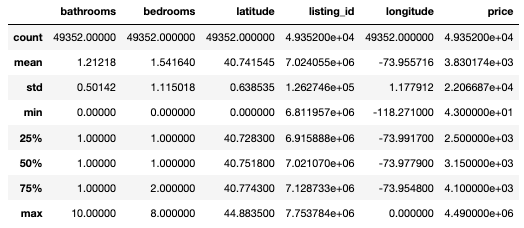
\includegraphics[width=300pt]{describe.png}
      \caption{Summary of numerical features}
      \label{fig:describe}
    \end{figure}
    \newpage
    The two dataframes are merged into a single dataframe for consistency. Afterwards additional steps like data cleaning and feature selection can be performed as well as engineering of features. We can extract with the help from pandas datetime modul new features from the date and time. In addition we can use word count techniques from the text feature.
      
    
    
	
	%\begin{table}
	%    \caption{Predicted link residual time and actual link failure time when node velocity is 2 m/sec}\label{tab2}
	%    \begin{tabular}{|l|l|l|}
	%        \hline
	%        Heading level &  Example & Font size and style\\
	%        \hline
	%        Title (centered) &  {\Large\bfseries Lecture Notes} & 14 point, bold\\
	%        1st-level heading &  {\large\bfseries 1 Introduction} & 12 point, bold\\
	%        2nd-level heading & {\bfseries 2.1 Printing Area} & 10 point, bold\\
	%        3rd-level heading & {\bfseries Run-in Heading in Bold.} Text follows & 10 point, bold\\
	%        4th-level heading & {\itshape Lowest Level Heading.} Text follows & 10 point, italic\\
	%        \hline
	%    \end{tabular}
	%    \end{table}
	
	\newpage
	\section{Methodology}
	In this chapter we discuss the methodology that has been applied to the given problem. It includes the steps for prepocessing the data in order to address any abnormalities or characteristics. Furthermore, it documents the implemented metrics, algorithms and techniques.
	
	\begin{figure}[h!]
      \centering
      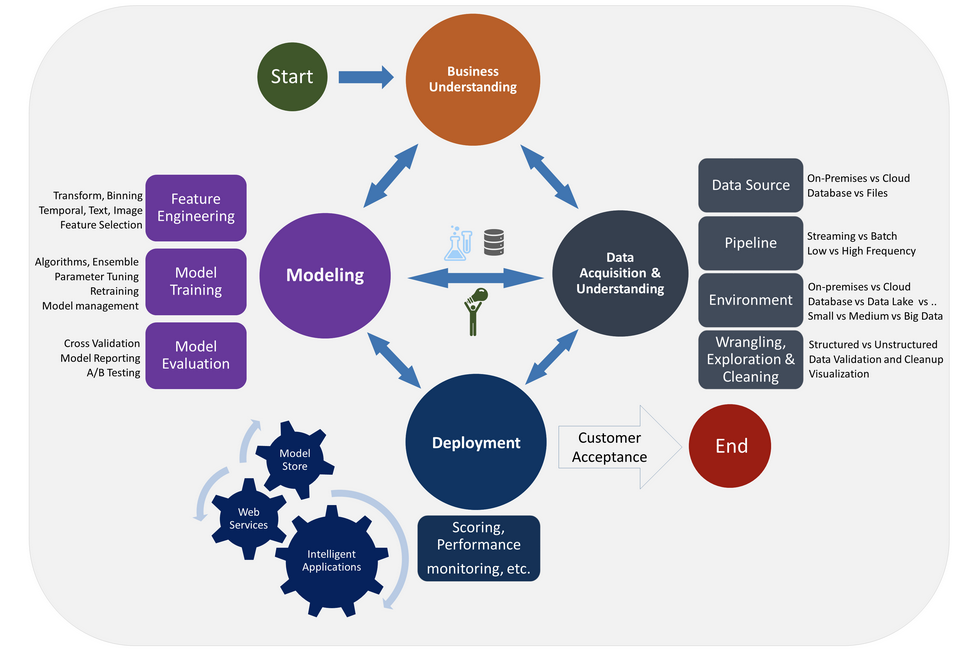
\includegraphics[width=300pt]{method.png}
      \caption{Data Science Lifecycle}
      \label{fig:data}
    \end{figure}
    
	\subsection{Exploratory Data Analysis}
	Before we begin to model the given problem, an analysis of the given data sets needs to be performed in order to understand which algorithms are going to be used in the next steps of the project. This section includes a data exploration which describes characteristic properties of the data as well as visualizations that help to summarize the most important outcomes. 
    \newline
    \newline
    As can be seen from the following figures, there are significantly more samples with low interest levels (35000) than medium (10000) and low (4000) interest levels. The map plotted with folium illustrates this observation quite well.
    
    
    \begin{figure}[h!]
      \centering
      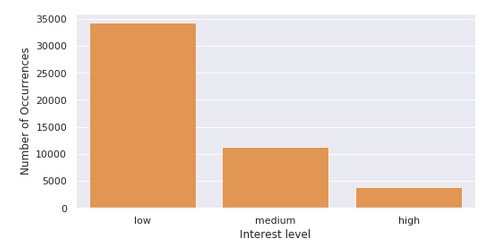
\includegraphics[width=250pt]{targetdist.png}
      \caption{Value Counts of target}
      \label{fig:data}
    \end{figure}
    
    \begin{figure}[h!]
      \centering
      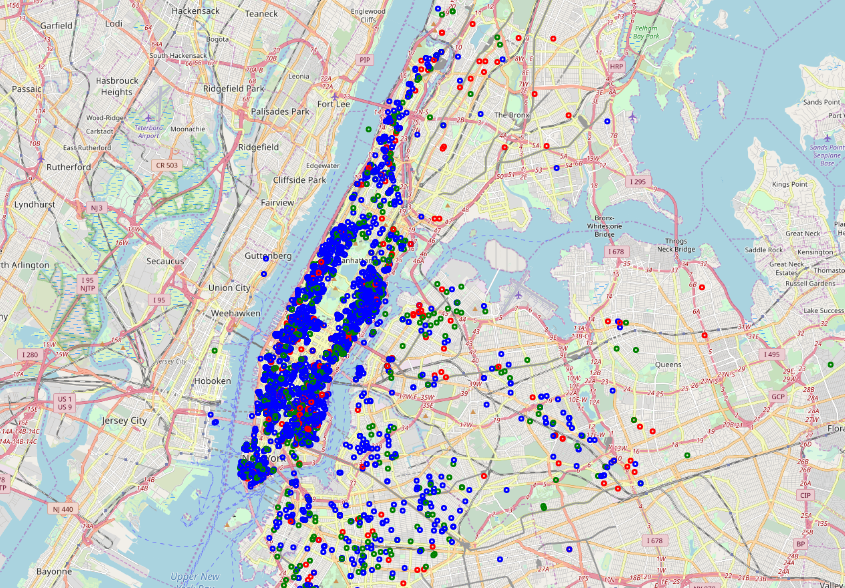
\includegraphics[width=250pt]{map.png}    
      \caption{Visual Representation of Interest lvl for NY}
      \label{fig:data}
    \end{figure}
    
    \newpage
    \subsection{Machine Learning Algorithms}
    
	\newpage
	\section{Results}
	
	\newpage
	\section{Discussion}
	fd

    moep moep
	\newpage
	\section{Conclusion}
	
	
	
	
	% ---- Bibliography ----
	%
	% BibTeX users should specify bibliography style 'splncs04'.
	% References will then be sorted and formatted in the correct style.
	%
	%\bibliographystyle{apalike}
	%\bibliography{mybib}
	%
	
\end{document}
